%%%%%%%%%%%%%%%%%%%%%%%%%%%%%%%%%%%%%%%%%
% Beamer Presentation
% LaTeX Template
% Version 1.0 (10/11/12)
%
% This template has been downloaded from:
% http://www.LaTeXTemplates.com
%
% License:
% CC BY-NC-SA 3.0 (http://creativecommons.org/licenses/by-nc-sa/3.0/)
%
%%%%%%%%%%%%%%%%%%%%%%%%%%%%%%%%%%%%%%%%%

%----------------------------------------------------------------------------------------
%	PACKAGES AND THEMES
%----------------------------------------------------------------------------------------

\documentclass[8pt]{beamer}
\usepackage{ctex}
\usepackage{xcolor}

\usepackage[utf8]{inputenc}
\usepackage{graphicx}
\usepackage{cmbright}
\usepackage{amsmath}
\usepackage{threeparttable}
\usepackage{tikz}
%\usefonttheme{professionalfonts}
%\setbeamertemplate{itemize/enumerate body begin}{\small} % 设置条目列表中的字体大小为 \small

\usefonttheme{serif}
% The Beamer class comes with a number of default slide themes
% which change the colors and layouts of slides. Below this is a list
% of all the themes, uncomment each in turn to see what they look like.

\usetheme{default}
%\usetheme{AnnArbor}
%\usetheme{Antibes}
%\usetheme{Bergen}
%\usetheme{Berkeley}			% 不错
%\usetheme{Berlin}
%\usetheme{Boadilla}				%跟Szeged很像
%\usetheme{CambridgeUS}  % 不错
%\usetheme{Copenhagen}
%\usetheme{Darmstadt}
%\usetheme{Dresden}         %跟Szeged很像
%\usetheme{Frankfurt}
%\usetheme{Goettingen}
%\usetheme{Hannover}      % 不错
%\usetheme{Ilmenau}
%\usetheme{JuanLesPins}
%\usetheme{Luebeck}
%\usetheme{Madrid}
%\usetheme{Malmoe}         %跟Szeged很像
%\usetheme{Marburg}
% \usetheme{Montpellier}   %跟Szeged很像
% \usetheme[width=2.5cm]{PaloAlto}
%\usetheme{Pittsburgh}
% \usetheme{Rochester}
%\usetheme{Singapore}
% \usetheme{Szeged}  % 点赞
% \usetheme{Warsaw}  % 点赞
% \setbeamertemplate{title page}[default][colsep=-4bp,rounded=false]

% Hide headline
\setbeamertemplate{headline}{}
\defbeamertemplate{footline}{myframe number}
{
  \hspace{1pt}
    \usebeamercolor[structure]{page number in head/foot}%
  \usebeamerfont{page number in head/foot}%
  \raisebox{1.7ex}[0pt][0pt]{% <--- change here
    \insertframenumber\,/\,\inserttotalframenumber\kern1em}%
}
\setbeamertemplate{footline}[myframe number]

\AtBeginSection[] % Displays outline at start of each section
{
	\begin{frame}<beamer>{Outline}
		\tableofcontents[currentsection, hideallsubsections]
	\end{frame}
}


% As well as themes, the Beamer class has a number of color themes
% for any slide theme. Uncomment each of these in turn to see how it
% changes the colors of your current slide theme.
%\definecolor{mycolor}{rgb}{.8,.0,.3}
%\setbeamercolor*{palette primary}{use=structure,fg=white,bg=mycolor}
%\usecolortheme{albatross}
%\usecolortheme{beaver}
%\usecolortheme{beetle}
%\usecolortheme{crane}
%\usecolortheme{dolphin}
%\usecolortheme{dove}
%\usecolortheme{fly}
%\usecolortheme{lily}
\usecolortheme{orchid}
% \usecolortheme{rose}
%\usecolortheme{seagull}
%\usecolortheme{seahorse}
%\usecolortheme{whale}
%\usecolortheme{wolverine}
%\usecolortheme[named=mycolor]{structure}
%\setbeamertemplate{footline} % To remove the footer line in all slides uncomment this line
%\setbeamertemplate{footline}[page number] % To replace the footer line in all slides with a simple slide count uncomment this line

%\setbeamertemplate{navigation symbols}{} % To remove the navigation symbols from the bottom of all slides uncomment this line


\usepackage{booktabs} % Allows the use of \toprule, \midrule and \bottomrule in tables

%----------------------------------------------------------------------------------------
%	TITLE PAGE
%----------------------------------------------------------------------------------------

\title{\songti 从强化学习到择时策略} % The short title appears at the bottom of every slide, the full title is only on the title page

\author{朱大福} % Your name
\institute[School of Economics (SOE)\\
Wang Yanan Institute for Studies in Economic \\ Xiamen University] % Your institution as it will appear on the bottom of every slide, may be shorthand to save space

\date{2024/07/09} % Date, can be changed to a custom date
\setbeamertemplate{itemize items}[default]
\setbeamertemplate{sidebar}[sidebar right]
% \definecolor{myco}{HTML}{a67678}
\definecolor{myco}{HTML}{8776a6}
\setbeamercolor{itemize item}{fg=myco} % all frames will have red bullets
\setbeamercolor{itemize subitem}{fg=myco} % all frames will have red bullets
% \setbeamercolor{block title}{bg=myco}
\setbeamercolor{structure}{fg=myco}
% \setbeamercovered{transparent}
\begin{document}
\songti
\begin{frame}
\titlepage % Print the title page as the first slide
\end{frame}
%
%\begin{frame}
%\frametitle{Overview} % Table of contents slide, comment this block out to remove it
%\tableofcontents[hideallsubsections] % Throughout your presentation, if you choose to use \section{} and \subsection{} commands, these will automatically be printed on this slide as an overview of your presentation
%\end{frame}

%----------------------------------------------------------------------------------------
%	PRESENTATION SLIDES
%----------------------------------------------------------------------------------------

%------------------------------------------------
% Sections can be created in order to organize your presentation into discrete blocks, all sections and subsections are automatically printed in the table of contents as an overview of the talk
%------------------------------------------------

 % A subsection can be created just before a set of slides with a common theme to further break down your presentation into chunks


%------------------------------------------------
%------------------------------------------------


\section{强化学习基本概念}
\begin{frame}

机器学习:Data-driven

\vspace{1em}

\frametitle{几类学习问题}
\begin{itemize}
\item 有监督学习
\begin{itemize}
\item Data: $(x,y)$
\item 目标:$x\rightarrow y$
\begin{figure}
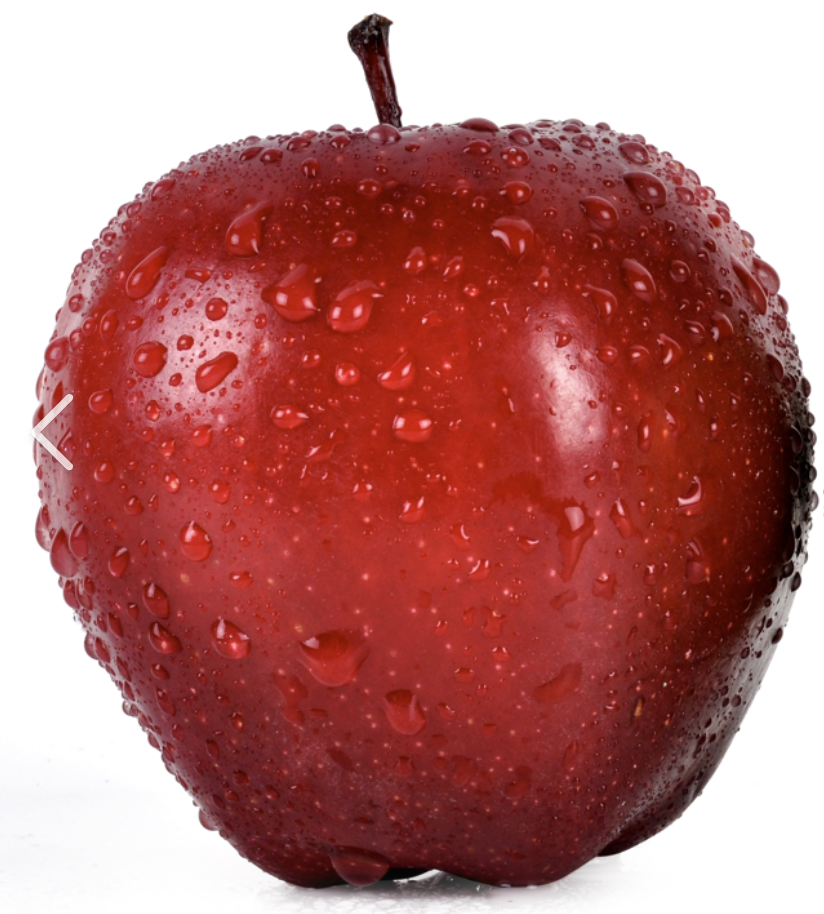
\includegraphics[height=3em]{../fig/apple1.png}

\end{figure}
\end{itemize}

\item 无监督学习
\begin{itemize}
\item Data: $x$
\item 目标:$x_1$和$x_2$是同类
\begin{figure}
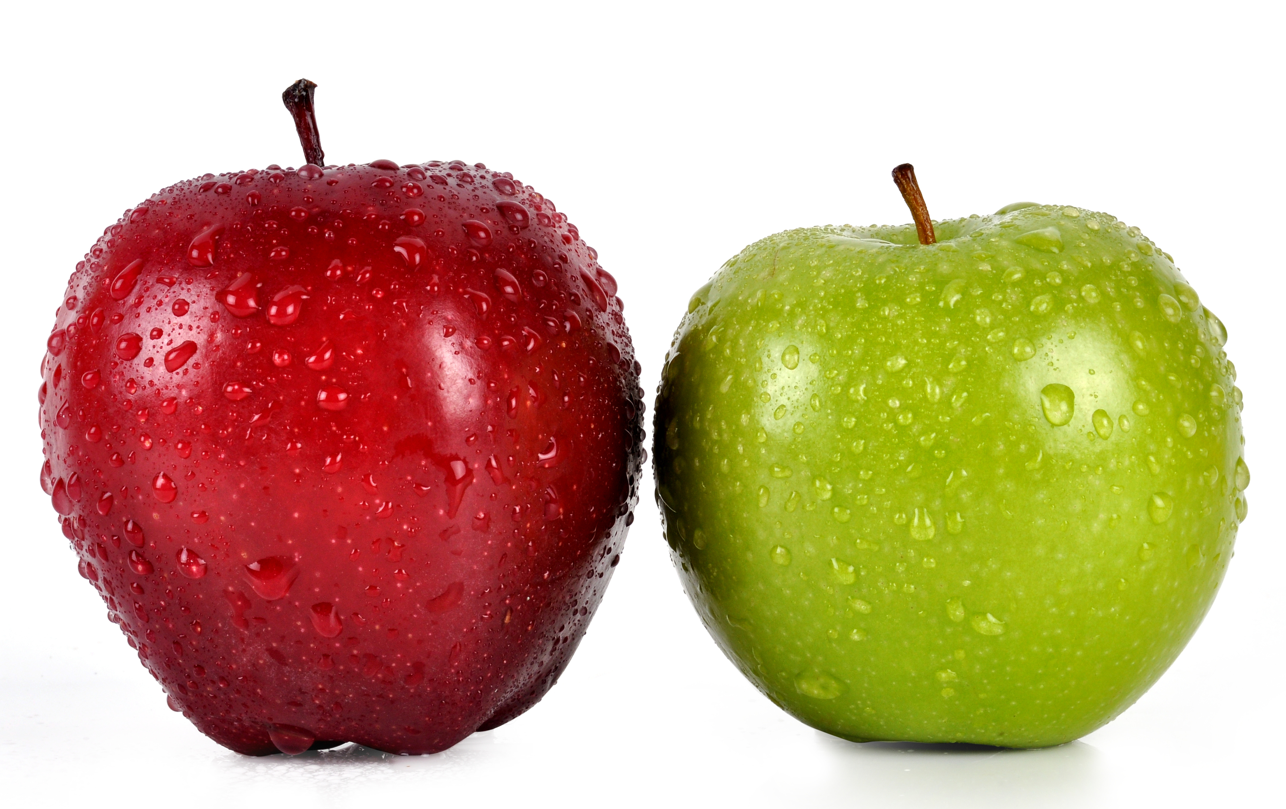
\includegraphics[height=3em]{../fig/apple2.png}

\end{figure}
\end{itemize}

\item 强化学习
\begin{itemize}
\item Data: $(s,a)$
\item 目标:回报最大化
\begin{figure}
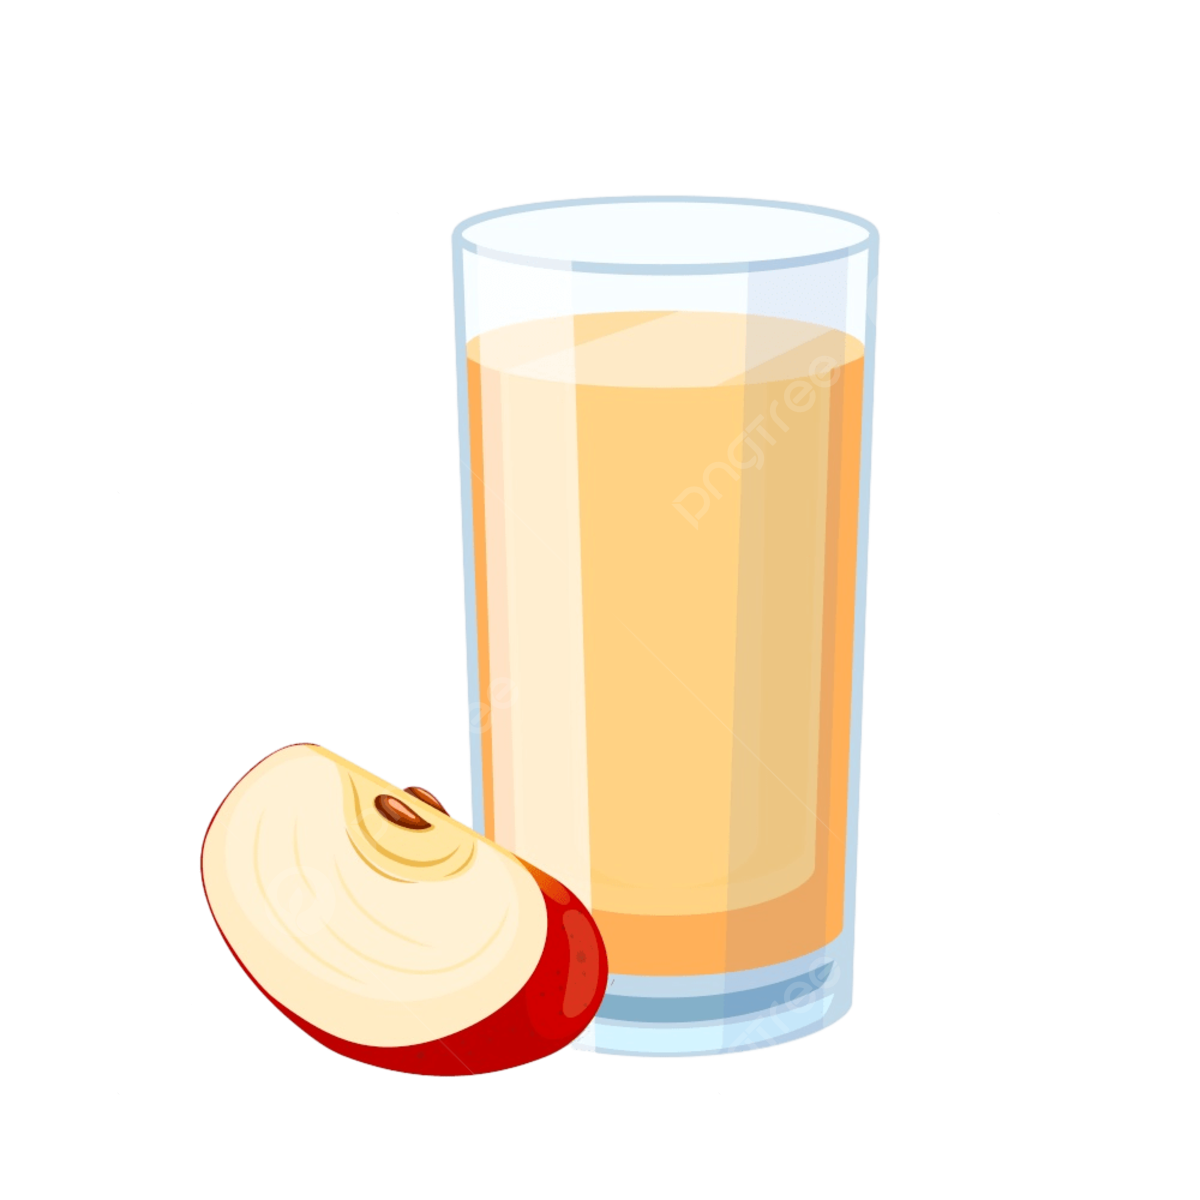
\includegraphics[height=6em]{../fig/apple3.png}

\end{figure}
\end{itemize}


\end{itemize}

\end{frame}

%------------------------------------------

\begin{frame}
\frametitle{Motivation}

有一家公司,怎样估值?\pause

\vspace{1em}

DCF模型(Discounted Cash Flow)

\[
DCF_t=CF_t+\frac{CF_{t+1}}{1+r}+\frac{CF_{t+2}}{(1+r)^2}+\cdots
\]

\pause

\vspace{1em}

记作 $G_t=DCF_t$, $R_t=CF_t$, $\gamma=1/(1+r)$

\[
\begin{aligned}
G_t&=R_t+\gamma R_{t+1}+\gamma^2 R_{t+2}+\cdots\\
&=R_t+\gamma (R_{t+1}+\gamma R_{t+2}+\cdots)
\end{aligned}
\]

\[
\therefore G_t=R_t+\gamma G_{t+1}
\]

\pause

公司的价值为

\[
V_t=\mathbb{E}[G_t]
\]

\vspace{1em}

Nothing special


\end{frame}

%------------------------------------------

\begin{frame}
\frametitle{状态(s),价值(V)}

假设公司有两种状态

\[
\mathcal{S}=\{\text{业绩好}, \text{业绩差}\}
\]


当前的状态为$S_t=s\in \mathcal{S}$。 

\vspace{1em}
显然业绩会影响公司的价值

\[
V(S_t=s)=\mathbb{E}[G_t|S_t=s]
\]

回忆$G_t=R_t+\gamma G_{t+1}$

\[
\therefore V(S_t=s)=\mathbb{E}[R_t|S_t=s]+\gamma V(S_{t+1}=s'|S_t=s)
\]

简写为

\[
V(s)=\mathbb{E}[R_t|s]+\gamma V(s'|s)
\]



\end{frame}

%------------------------------------------

\begin{frame}
\frametitle{Markov Decision Process}

马尔可夫决策过程(MDP):下一刻的状态只和当前时刻有关

\[
P(S_{t+1}|S_t,S_{t-1},\cdots)=P(S_{t+1}|S_t)=P(s'|s)
\]

\vspace{1em}

公司$t+1$期的业绩情况只和$t$期有关,状态转移用概率表示,比如 $P(S_{t+1}=\text{业绩好}|S_t=\text{业绩差}),\cdots$

\[
\begin{aligned}
V(s'|s)&=P(\text{好}|s)\cdot V(\text{好})+P(\text{差}|s)\cdot V(\text{差})\\
&=\sum_{s'\in \mathcal{S}}P(s'|s)\cdot V(s')
\end{aligned}
\]

\end{frame}


\begin{frame}
\frametitle{动作(a)}

作为公司老板,你的目标是什么\pause

\vspace{1em}

你能做的事情是

\[
\mathcal{A}=\{\text{研发}, \text{不研发}\}
\]

策略是

\[
\pi(\text{研发}|\text{好})=p,\quad \pi(\text{不研发}|\text{好})=1-p
\]

\[
\pi(\text{研发}|\text{差})=q,\quad \pi(\text{不研发}|\text{差})=1-q
\]

\vspace{1em}

我们很好奇$p=?,q=?$

\end{frame}


\begin{frame}
\frametitle{动作(a)}

回顾

\[
V(s)=\mathbb{E}[R_t|s]+\gamma V(s'|s)
\]

\[
V(s'|s)=\sum_{s'\in \mathcal{S}}P(s'|s)\cdot V(s')
\]

\pause

$\Rightarrow$

\[
V(s)=\mathbb{E}[R_t|s]+\gamma\cdot \left[\sum_{s'\in \mathcal{S}}P(s'|s)\cdot V(s')\right]
\]

$a$会影响谁?

\pause

\[
\mathbb{E}[R_t|s]\rightarrow \mathbb{E}[R_t|s,a]
\]

\[
P(s'|s)\rightarrow P(s'|s,a)
\]

\[
V(s)\rightarrow V(s|a)
\]


\end{frame}

\begin{frame}
\frametitle{动作价值函数(Q)}

\[
V(s)=\mathbb{E}[R_t|s]+\gamma\cdot \left[\sum_{s'\in \mathcal{S}}P(s'|s)\cdot V(s')\right]
\]

\[
\Downarrow
\]

\[
V(s|a)=\mathbb{E}[R_t|s,a]+\gamma\cdot \left[\sum_{s'\in \mathcal{S}}P(s'|s,a)\cdot V(s')\right]
\]

\pause

定义

\[
Q(s,a)=V(s|a)
\]

\end{frame}

\begin{frame}
\frametitle{动作价值函数(Q)}

\[
V(\text{好})=\pi(\text{研发}|\text{好})Q(\text{好}, \text{研发})+\pi(\text{不研发}|\text{好})Q(\text{好},\text{不研发})
\]

\pause

\[
V(s)=\sum_{a\in \mathcal{A}}\pi(a|s)Q(s,a)
\]

\pause

\[
Q(s,a)=\mathbb{E}[R_t|s,a]+\gamma\cdot \left[\sum_{s'\in \mathcal{S}}P(s'|s,a)\cdot V(s')\right]
\]

\pause

\[
Q(s,a)=\mathbb{E}[R_t|s,a]+\gamma\cdot \left[\sum_{s'\in \mathcal{S}}P(s'|s,a)\cdot \sum_{a'\in \mathcal{A}}\pi(a'|s')Q(s',a')\right]
\]

\end{frame}

\begin{frame}
\frametitle{随机性的两个来源}

\[
Q(s,a)=\mathbb{E}[R_t|s,a]+\gamma\cdot \left[\sum_{s'\in \mathcal{S}}P(s'|s,a)\cdot \sum_{a'\in \mathcal{A}}\pi(a'|s')Q(s',a')\right]
\]

\vspace{1em}

\begin{enumerate}
\item 状态s下,做什么动作a?

\[
\pi(a|s)
\]

\item 状态s下且做出动作a,会到达什么状态s'?

\[
P(s'|s,a)
\]
\end{enumerate}


\end{frame}

\section{Q-learning}
\begin{frame}
\frametitle{最优化问题}

\[
Q(\text{业绩好},\text{研发})=130, \quad Q(\text{业绩好},\text{不研发})=-50
\]





\end{frame}




\end{document} 